% Created 2016-11-08 Tue 15:04
% Intended LaTeX compiler: pdflatex
\documentclass[xcolor={usenames,dvipsnames}]{beamer}
\usepackage[utf8]{inputenc}
\usepackage[T1]{fontenc}
\usepackage{graphicx}
\usepackage{grffile}
\usepackage{longtable}
\usepackage{wrapfig}
\usepackage{rotating}
\usepackage[normalem]{ulem}
\usepackage{amsmath}
\usepackage{textcomp}
\usepackage{amssymb}
\usepackage{capt-of}
\usepackage{hyperref}
\usepackage{geometry}
\usepackage[activate={true,nocompatibility},final,tracking=true,kerning=true,spacing=nonfrench,factor=1100,stretch=10,shrink=10]{microtype}
\usepackage{minted}
\usepackage{svg}
\usepackage{tikz}
\usepackage{amsmath}
\usepackage[backend=biber,style=alphabetic]{biblatex}
\fvset{fontsize=\footnotesize}
\fvset{frame=lines}
\fvset{framesep=5pt}
\AtBeginSection[]{\begin{frame}<beamer>\frametitle{Outline}\tableofcontents[currentsection]\end{frame}}
\beamertemplatenavigationsymbolsempty
\setbeamertemplate{footline}[frame number]
\DeclareUnicodeCharacter{200B}{}
\addbibresource{~/Documents/ms/thesis/thesis.bib}
\usetheme{default}
\author{Zhitao Gong}
\date{\today}
\title{RFID-Based Indoor Spatial Query Evaluation with Bayesian Filtering Techniques}
\hypersetup{
      pdfauthor={Zhitao Gong},
      pdftitle={RFID-Based Indoor Spatial Query Evaluation with Bayesian Filtering Techniques},
      pdfkeywords={},
      pdfsubject={},
      pdfcreator={Emacs 24.5.1 (Org mode 9.0)},
      pdflang={English},
      bookmarks=true,
      unicode=true,
      pdftoolbar=true,
      pdfmenubar=true,
      pdffitwindow=false,
      pdfstartview={FitH},
      pdfnewwindow=true,
      colorlinks=true,
      linkcolor=Maroon,
      citecolor=ForestGreen,
      filecolor=Mulberry,
      urlcolor=MidnightBlue}
\begin{document}

\maketitle

\section{Introduction}
\label{sec:orga4bafcc}

\begin{frame}[label={sec:org0b88da1}]{Motivation}
\alert{Goal} -- Cleanse noisy RFID readings for indoor spatial queries.
\end{frame}

\begin{frame}[label={sec:org1ded071}]{Existing Solutions}
\begin{itemize}
\item \cite{jensen2009-graph}
\item \cite{yang2009-scalable}
\item \cite{yang2010-probabilistic}
\item \cite{ku2013-bayesian}
\end{itemize}
\end{frame}

\section{Preliminary}
\label{sec:org008e991}

\begin{frame}[label={sec:org21016dd}]{Particle Filter}
\end{frame}

\begin{frame}[label={sec:org569329f}]{Kalman Filter}
\end{frame}

\section{System}
\label{sec:org704f548}

\begin{frame}[label={sec:org913720d}]{Overview}
\begin{center}
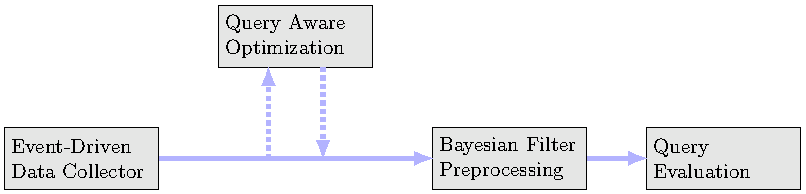
\includegraphics[width=.9\linewidth]{img/system-design.pdf}
\end{center}

\begin{description}
\item[{Data Collector}] generates ground truth data.
\item[{Query Optimization}] filters out \emph{non-candidates}.
\item[{Bayesian Filters}] cleanse the noisy RFID data.
\item[{Query Evaluation}] answers spatial queries.
\end{description}
\end{frame}

\begin{frame}[label={sec:orge3859bb}]{Event-Driven Data Collector}
\begin{center}
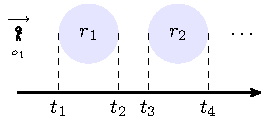
\includegraphics[width=.9\linewidth]{img/data-collector.pdf}
\end{center}

The data collected is
\[o_1: (t_1, r_1), (t_2, \text{NIL}), (t_3, r_2), (t_4, \text{NIL}),
   \dots\]
\end{frame}

\begin{frame}[label={sec:org5a90db8}]{Optimization Model}
\begin{center}
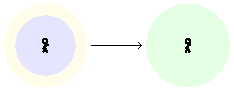
\includegraphics[width=.7\textwidth]{img/uncertainty.pdf}
\end{center}

We are pruning \emph{non-candidates} by their uncertainty range.
\begin{itemize}
\item \tikz\fill[blue!20] circle [radius=.5em]; denotes the reader
range.
\item \tikz\fill[green!20] circle [radius=.5em]; denotes the
uncertainty range.
\end{itemize}
\end{frame}

\begin{frame}[label={sec:org19a8b6c}]{Optimization Model -- Range Query}
\begin{center}
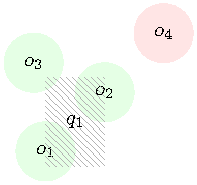
\includegraphics[width=.5\textwidth]{img/range-filter.pdf}
\end{center}

The candidate set is \(\{o_1, o_2, o_3\}\)
\end{frame}

\begin{frame}[label={sec:org2d6d1c0}]{Optimization Model -- \(k\)NN Query}
\begin{center}
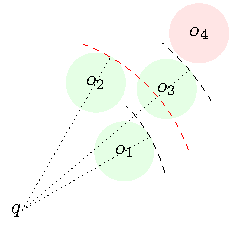
\includegraphics[width=.5\textwidth]{img/knn-filter.pdf}
\end{center}

The candidate set for 2NN query \(\{o_1, o_2, o_3\}\).
\end{frame}

\begin{frame}[label={sec:org4f29f69}]{Bayesian Filtering}
\begin{columns}
\begin{column}{0.5\columnwidth}
\begin{center}
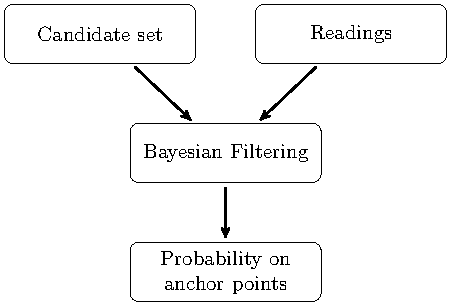
\includegraphics[width=.9\linewidth]{img/bayesian-filter.pdf}
\end{center}
\end{column}

\begin{column}{0.5\columnwidth}
\begin{enumerate}
\item Object are restricted on walking graph for simplicity.
\item Each object/particle in the candidate set is mapped to the
nearest \emph{anchor point}.  Information associated with each
anchor point \(\{(o_1, 0.14), (o_2, 0.03), \dots\}\)
\end{enumerate}
\end{column}
\end{columns}
\end{frame}

\begin{frame}[label={sec:orge5e3b0b}]{Evaluation Module}
\begin{center}
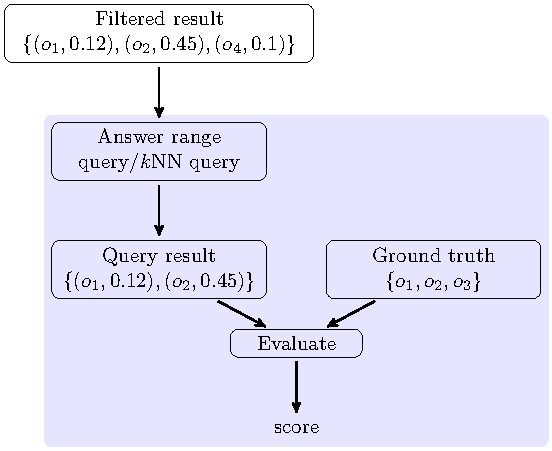
\includegraphics[width=.9\textwidth]{img/evaluation.pdf}
\end{center}
\end{frame}

\section{Experiment}
\label{sec:org7753fc0}

\begin{frame}[label={sec:orge7c68c3}]{Range Query Window Size}
\begin{enumerate}
\item KL value lower is better.
\item Query window size is the ratio of areas between query window and
totally environment.
\end{enumerate}

\begin{center}
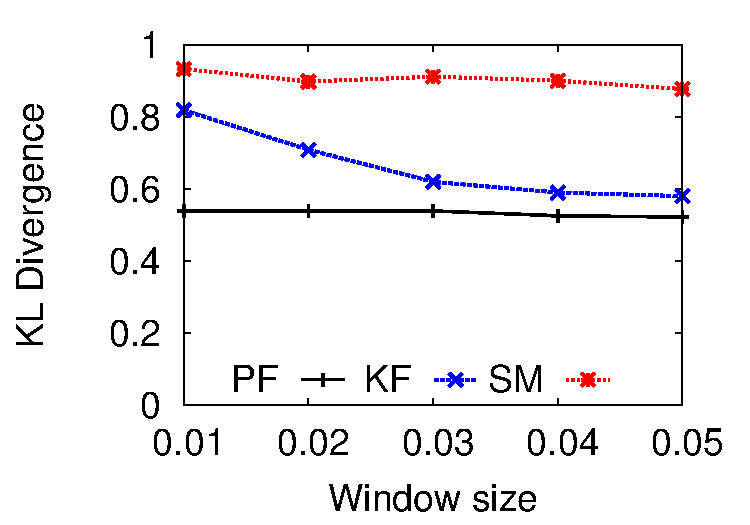
\includegraphics[width=.7\textwidth]{img/kl-w.pdf}
\end{center}
\end{frame}

\begin{frame}[label={sec:orge5fa32d}]{\(k\) in \(k\)NN}
\begin{enumerate}
\item Hit rate higher is better.
\item \(k\) is the number of nearest neighbors.
\end{enumerate}

\begin{center}
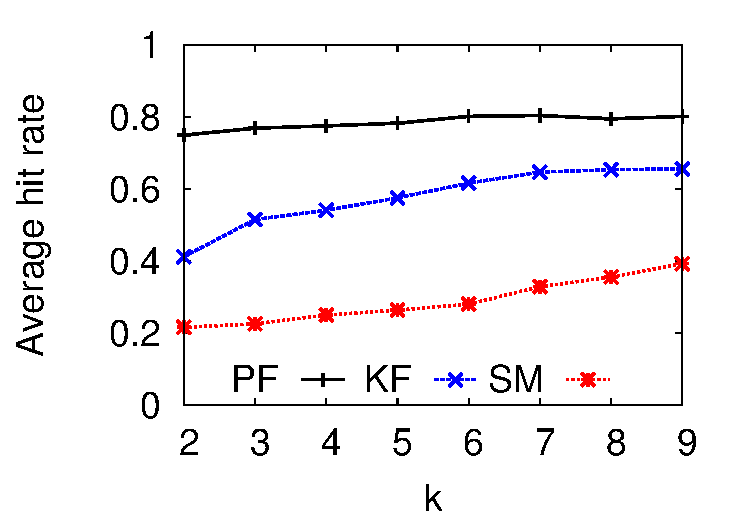
\includegraphics[width=.7\textwidth]{img/hit-k.pdf}
\end{center}
\end{frame}

\begin{frame}[label={sec:orge5ccc0f}]{Number of Particles}
\begin{enumerate}
\item KL value lower is better.
\item This parameter only applies to particle filter.
\end{enumerate}

\begin{center}
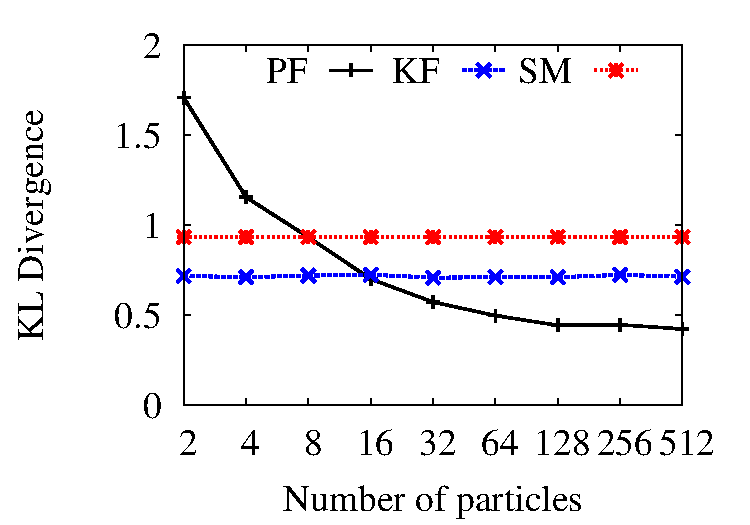
\includegraphics[width=.7\textwidth]{img/kl-p.pdf}
\end{center}
\end{frame}

\begin{frame}[label={sec:org674a560}]{Number of Moving Objects}
\begin{enumerate}
\item KL value lower is better.
\item Total number of objects in the environment.
\end{enumerate}

\begin{center}
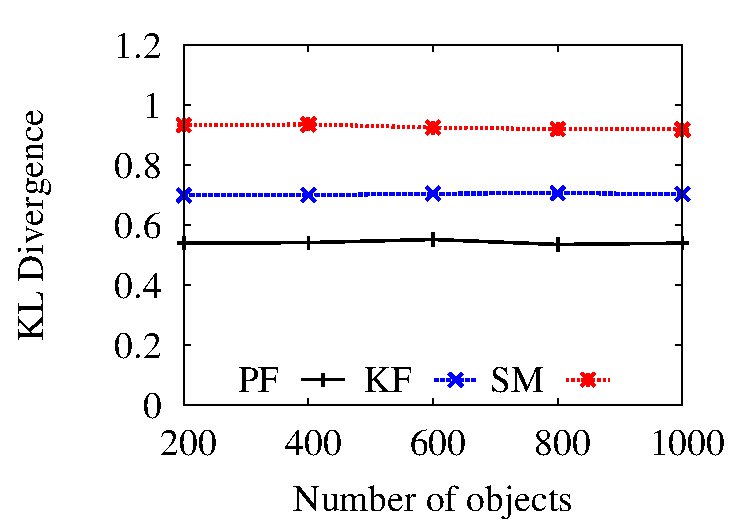
\includegraphics[width=.7\textwidth]{img/kl-n.pdf}
\end{center}
\end{frame}

\begin{frame}[label={sec:org7cfd852}]{Detection Range}
\begin{enumerate}
\item KL value lower is better.
\item The detection range of each reader.
\end{enumerate}

\begin{center}
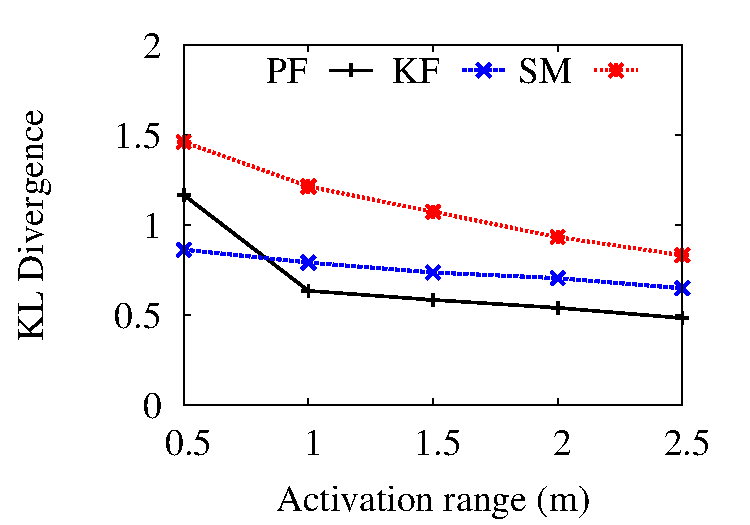
\includegraphics[width=.7\textwidth]{img/kl-r.pdf}
\end{center}
\end{frame}

\begin{frame}[label={sec:orgc7032ea}]{Change of Volume}
Suppose \(t_1\) the result set is \(\{o_1, o_2, o_3\}\), and
\(t_2\) the result changes to \(\{o_1, o_2, o_4\}\), then the
change volume is 2.

\begin{center}
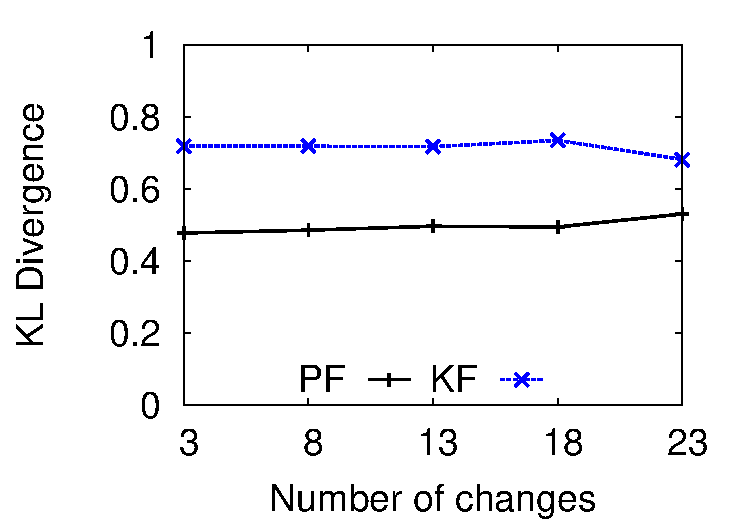
\includegraphics[width=.7\textwidth]{img/cont-kl-n.pdf}
\end{center}
\end{frame}

\begin{frame}[label={sec:orga6452b5}]{Query Duration}
Measure how stable our algorithm is.

\begin{center}
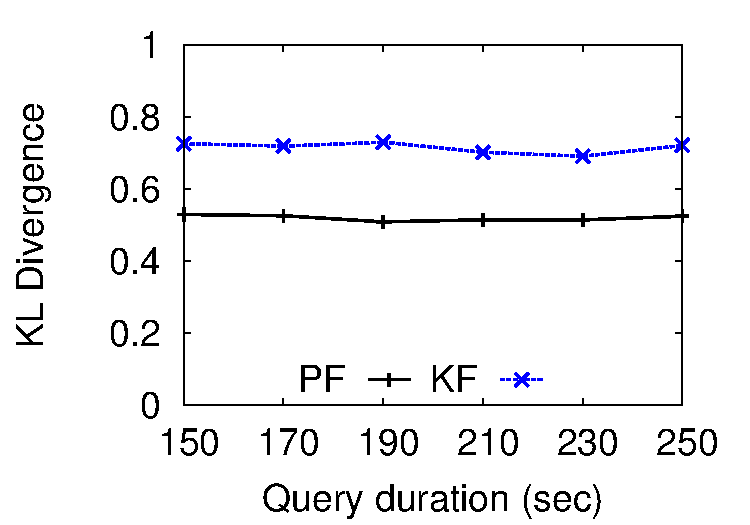
\includegraphics[width=.7\textwidth]{img/cont-kl-t.pdf}
\end{center}
\end{frame}

\section{Discussion}
\label{sec:org5022c45}

\begin{frame}[label={sec:org7841d58}]{Summary}
\begin{enumerate}
\item We designed Bayesian-filter algorithms for RFID data cleansing.
\item We propose indoor walking graph model and anchor point model to
simplify the filter process.
\item We propose two metrics to evaluate continuous queries.
\item Through extensive experiment on range query and \(k\)NN, we
demonstrate the effectiveness of our solutions compared with
symbolic-model.
\end{enumerate}
\end{frame}

\begin{frame}[label={sec:orgbee18f5}]{Future Work}
\end{frame}
\end{document}